\chapter{Platforma Android}
\section{Istoric}
\vspace{1cm}
\begin{defn}Android este o platformă software și un sistem de operare pentru dispozitive mobile precum smartphone-uri și tablete, bazată pe nucleul Linux, dezvoltată inițial de compania Google, iar mai târziu de consorțiul comercial Open Handset Alliance\cite{5}. 
\end{defn}
Android permite dezvoltatorilor să scrie cod gestionat în limbajul Java, controlând dispozitivul prin intermediul bibliotecilor Java dezvoltate de Google\cite{6}. \newline
Aplicațiile scrise în C și în alte limbaje pot fi compilate în cod mașină ARM și executate, dar acest model de dezvoltare nu este sprijinit oficial de către Google\cite{7}\cite{8}. \newline
\bigskip

 Lansarea platformei Android în data de 5 noiembrie 2007 a fost anunțată prin fondarea Open Handset Alliance, un consorțiu de 48 de companii de hardware, software și de telecomunicații, consacrat dezvoltării de standarde deschise pentru dispozitive mobile. Google a lansat cea mai mare parte a codului Android sub licența Apache, o licență de tip free-software și open source.\cite{5}

\section{Arhitectura platformei}
Android se bazează pe tehnologii variate open source pentru a pune la dispoziție o platformă mobilă solidă ce poate satisface toate necesitățile unui utilizator/dezvoltator.\newline Arhitectura platformei poate fi cel mai bine descrisă ca o serie de 5 niveluri principale, fiecare corespunzând unei operațiuni de bază. \newpageÎn imaginea anterioară se poate observa arhitectura platformei Android, care cuprinde cele 5 niveluri principale și subcomponentele acestora.\cite{1}
\begin{figure}
\caption{Arhitectura platformei}
\begin{center}
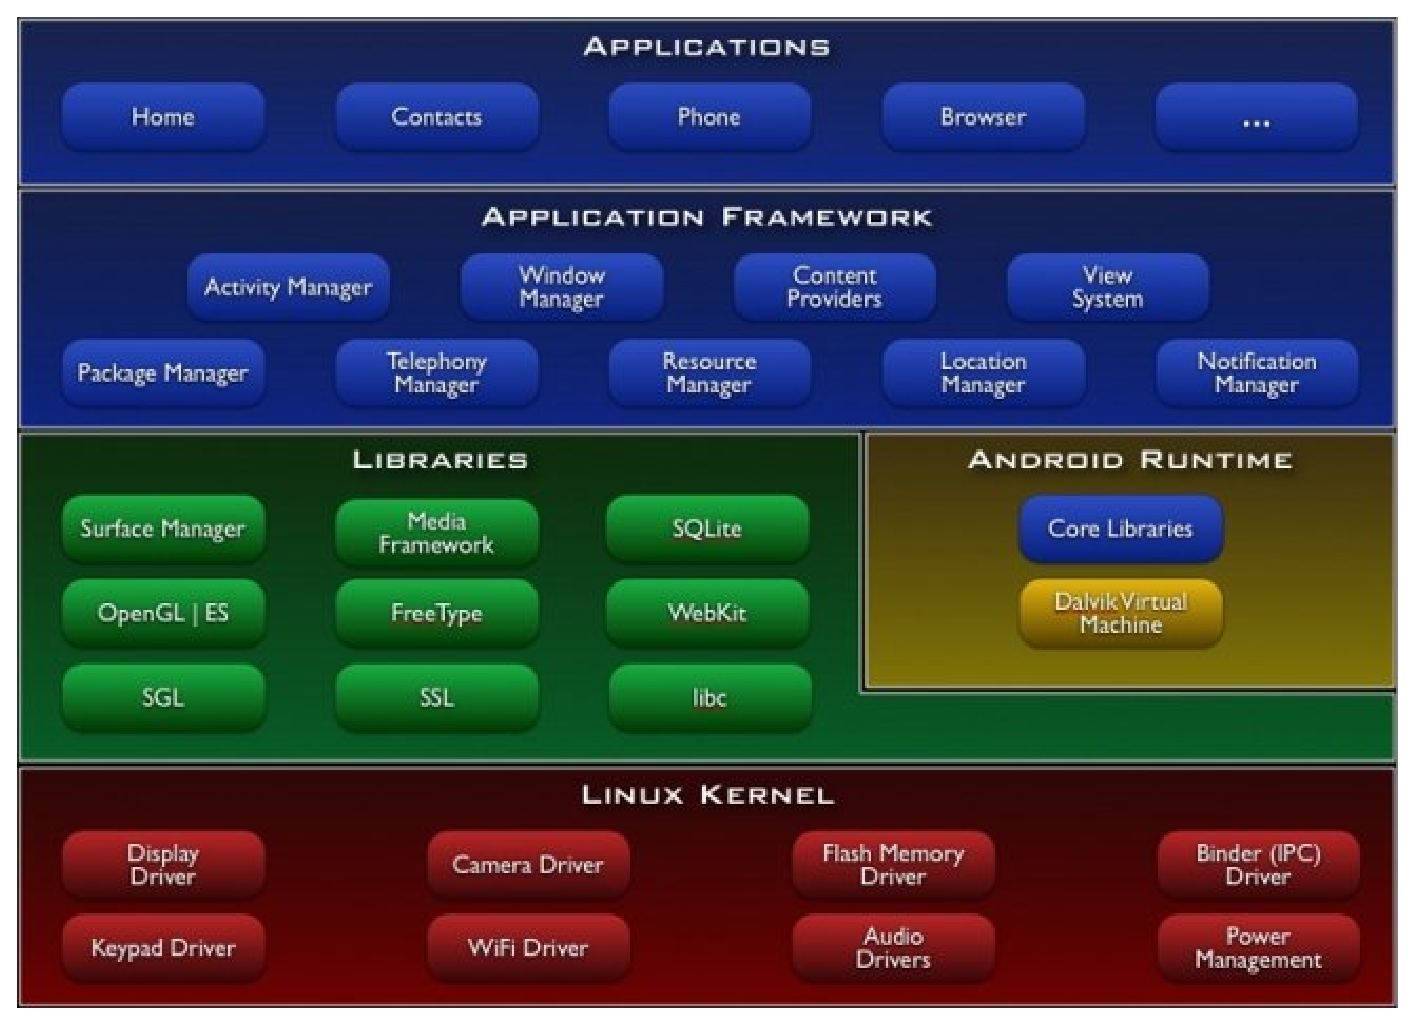
\includegraphics[width=0.9\textwidth]
{imagini/arhitectura-sistem.eps}
\end{center}
\end{figure}

\section{Linux Kernel}
\vspace{1cm}
Nivelul de bază al platformei Android este Linux kernel, acesta utilizându-se de binecunoscutul Linux kernel pentru a furniza funcționalitatea sistemului de operare.\newline


 Pentru a satisface nevoile dispozitivelor mobile, nucleul Linux pe care se bazează Android a suferit schimbări arhitecturale. Cele mai notabile fiind cele ce vor fi prezentate în următoarea secțiune.\newline
\newpage
\textbf{Binder}\newline
Arhitectura platformei Android se folosește intens de comunicația între procese (inter-process communication-IPC). Aplicațiile comunică cu sistemul, telefonul, serviciile și între ele utilizând IPC. Având în vedere că mecanismul IPC furnizat de sistemul de operare Linux nu este suficient, platforma Android a dezvoltat propriul sistem IPC, cunoscut sub numele de Binder, acesta fiind canalul central de comunicație al întregii platforme Android.\newline 
Deoarece Binder este implementat ca un serviciu de bază in Linux kernel Android, dezvoltatorii de aplicații nu interacționează direct cu acesta. Majoritatea API-urilor \footnote{application programming interfaces } frameworkului Android se bazează pe Binder pentru a interacționa cu platforma într-un mod transparent dezvoltatorului de aplicații.\newline
 Pentru a utiliza Binder în interacționarea cu alte aplicații din sistem, SDK-ul Android \footnote{Android Software Development Kit } furnizează  Android Interface Definition Language (AIDL).  AIDL cuprinde funcționalitatea de a descompune obiectele primite în primitive astfel încât Binder le poate înțelege și utiliza dincolo de limitele procesului.\cite{2}\newline

\textbf{Logger}\newline
Logger este mecanismul esențial pentru depanare. Având în vedere faptul că aplicațiile mobile depind mult de elemente din mediul înconjurător cum ar fi rețelele WiFi și de datele care provin de la anumiți senzori ai dispozitivului, funcționalitățile de logare ale aplicației nu sunt îndeajuns de bune pentru probleme complexe. De aceea, este esențial să combinăm funcționalitățile de logare ale sistemului cu cele ale aplicației pentru o imagine complexă.\newline 
Acest lucru devine mai greu de obținut atunci când dezvoltarea aplicației și executarea acesteia au loc pe mașini diferite.\newline
Android furnizează un sistem larg de servicii de logare care agreghează logările care provin din partea platformei Android și cele care provin de la aplicațiile care rulează pe aceasta.\newline 
SDK-ul Android-ului furnizează de asemenea uneltele necesare pentru a monitoriza logările în timp real și suport pentru filtrare avansată.\cite{2}\newline

\textbf{Wake Locks}\newline
Platforma Android este dezvoltată pentru a opera pe dispozitive mobile cu resurse limitate. Puterea bateriei este cea mai importantă și de aceea, dispozitivele Android intră in modul low-powered, numit și sleep. Chiar dacă acest mod permite utilizarea rezervei de baterie rămasă într-un mod eficient, nu este indicat ca un dispozitiv să intre în modul sleep pe parcursul unei operațiuni importante ale unei aplicații sau a unui serviciu.\newline
 Wake locks au fost introduse în Linux kernel al platformei Android cu scopul de a preveni aplicațiile de la intrarea in modul sleep.\cite{2}\newline

\textbf{Alarm Timer\footnote{în română, cronometru}}\newline
La fel cum am menționat anterior în secțiunea ,,Wake Locks'', dispozitivele intră în modul sleep pentru a conserva puterea bateriei. Pe parcursul modului sleep, nicio aplicație Android nu poate rula. Din acest motiv, a fost introdus alarm timer-ul care permite aplicațiilor să programeze sarcinile de execuție. \cite{2}\newline

\textbf{Low Memory Killer}\newline
La fel ca și bateria, memoria este de asemenea o resursă limitată a dispozitivelor mobile. Pe lângă dimensiunea memoriei, încărcarea în memorie a aplicațiilor este de asemenea o operație costisitoare. Pentru a rezolva aceasta problemă, platforma Android menține toate aplicațiile deschise încărcate în memorie chiar dacă utilizatorul nu mai interacționează cu ele.\newline
 Acest lucru permite utilizatorului o interschimbare rapidă între aplicații.\newline
 Această optimizare vine însă cu un cost: dispozitivul poate rămâne repede fără memorie dacă mai multe aplicații sunt deschise. \newline
 Low Memory Killer cunoscut și ca Viking Killer, a fost introdus în Linux kernel al platformei Android pentru a administra și a revendica memoria înainte ca dispozitivul să rămână fără aceasta.\newline
 Atunci când memoria disponibilă scade sub un anumit prag, low memory killer, elimină din memorie aplicațiile pornite, începând cu cele mai puțin importante.\newline
 Importanța unei aplicații este definită după vizibilitatea acesteia pentru utilizator.\newline
 O aplicație care rulează în prim plan este considerată cea mai importantă iar o aplicație care rulează pe fundal nu este considerată importantă. Stările curente ale aplicațiilor închise sunt salvate și pot fi reluate când utilizatorul se întoarce la o aplicație.\cite{2}\newline


\textbf{File System}\newline
Platforma Android se bazează pe Yet Another Flash File System (YAFFS2) ca și tip primar de sistem de fișiere, fiind dezvoltat pentru a lucra pe NAND-based flash chips. Sistemul de fișiere Android este de asemenea structurat într-un mod specific pentru a fi posibilă o actualizare ușoară a unor porțiuni ale platformei, aceste modificări neavând impact asupra celorlalte părți. Acest lucru este realizat prin menținerea porțiunilor platformei Android în partiții de sistem diferite, astfel garantându-se și o securitate mai ridicată întrucât componentele cheie ale platformei nu sunt mutabile pe parcursul rulării, evitând infectarea cu viruși și malware a componentelor cheie ale sistemului de operare.\cite{2}\newpage

Partițiile utilizate depind de producătorii dispozitivelor, cele mai des întâlnite fiind următoarele:\newline
\begin{itemize}
  \item /boot
  \item /system
  \item /recovery
	\item /data
	\item /cache
\end{itemize}

\section{Native Libraries}
\vspace{1cm}
Pe nivelul superior nucleului Linux, platforma Android conține un set de biblioteci native, precum:
\begin{itemize}
\item SQLite: Furnizează o memorie internă ce relaționează cu o bază de date SQL pentru persistența datelor și accesarea rapidă a acestora într-un mod structurat
\item WebKit:  Furnizează suport de interpretare HTML/CSS  și un motor de executare JavaScript pentru a permite aplicațiilor Android să încorporeze tehnologii web
\item OpenGL ES: Furnizează funcționalități performante pentru grafica 2D si 3D
\item Open Core: Furnizează un framework media care permite aplicațiilor Android să înregistreze și să redea conținut audio și video
\item Open SSL: Furnizează protocoalele Secure Socket Layer (SSL)  și Transport Level Security (TLS) care permit aplicațiilor Android să comunice în mod securizat cu servicii la distanță prin utilizarea criptografiei
\end{itemize}\cite{1}

\section{Android Runtimes}
\vspace{1cm}
Android Runtime este porțiunea care dirijează platforma Android, rulând atât serviciile platformei cât și aplicațiile care rulează pe platformă.\newline

\textbf{Android Runtime (ART)}
\newline
Limbajul de programare oficial folosit pentru Android este Java. Java este un limbaj de programare obiect-orientat specific dezvoltării de aplicații independente de platforma de lucru.
Acest lucru este posibil deoarece codul Java compilat al aplicației este realizat într-un limbaj independent de platformă numit bytecode. Acest bytecode este executat de Java Virtual Machine care rulează pe platformă.\newline

The Android Runtime (ART) este noul Java Virtual Machine ce a fost introdus într-un mod experimental în versiunea de Android 4.4, ca mai apoi să fie introdus în versiunea Android 5.0 ca runtime-ul oficial al aplicațiilor Android.  Înainte de versiunea 5.0, aplicațiile Android rulau pe Dalvik Virtual Machine (VM).\newline
În comparație cu abordarea Dalvik VM’s just-in-time (JIT) , ART se bazează pe o abordare ahead-of-time (AOT) , care permite compilarea codului bytecode și translatarea lui în cod mașină pe timpul instalării aplicației. Acest lucru permite codului aplicației să fie executat în viitor direct din mediul de rulare al dispozitivului.\cite{1}\newline

\section{Android Applications}
\vspace{1cm}
\textbf{Compiled Android Applications}\newline
Chiar dacă oficial ART este runtime-ul utilizat pentru platforma Android începând cu versiunea 5.0, majoritatea dispozitivelor Android care rulează pe versiuni mai vechi de Android utilizează plaforma Dalvik VM. \newline
Pentru a produce pachete de aplicații care să fie compatibile atât cu ART cât și cu Dalvik VM, acestea sunt încă dezvoltate utilizând specificațiile Dalvik. \newline Deoarece a fost optimizat pentru dispozitive mobile, Dalvik VM procesează doar un tip special de bytecod numit Dalvik Executable (DEX). SDK-ul Androidului cuprinde unelte care pot traduce bytecode-ul standard din Java în bytecode DEX pe parcursul asamblării aplicației android. Utilizarea bytecode-ului DEX furnizează multe avantaje în comparație cu bytecode-ul standard Java. Art realizează conversia automată de la formatul Dalvik DEX la formatul ART OAT imediat după instalarea aplicației pe dispozitiv.\cite{1}\newline


\textbf{Application Sandbox}\newline
Platforma Android este construită având în vedere securitatea ca o necesitate importantă. Astfel rulează fiecare aplicație într-un sandbox izolând datele aplicației și codul executabil de alte aplicații.\newline
- Fiecare aplicație rulează pe instanța ART VM dedicată. \newline
- Datele aplicației sunt protejate prin utilizarea unui fișier cu permisiuni ale sistemului. Fiecare aplicație are asignat un cont la instalare și sistemul de operare restricționează accesul la date pentru acel cont.\newline
- Aplicațiile pot să comunice cu sistemul sau cu alte aplicații prin interfața de comunicare pe care platforma Android o pune la dispoziție. Aceste interfețe sunt de asemenea protejate prin permisiuni Android\cite{1}.\newline

\textbf{Application Framework}\newline
Framework-ul aplicației rulează pe ART VM și dispune de o interfață pentru ca aplicațiile Android să interacționeze cu platforma Android și cu dispozitivul mobil. Cuprinde servicii precum : Package Manager, Telephony Manager, Location Manager, and Notifications Manager.\cite{1}\newline


\textbf{Applications}\newline
Spațiul aplicațiilor cuprinde toate aplicațiile Android cu care se confruntă utilizatorul care rulează pe ART VM. Aceste aplicații includ și aplicațiile de la terți, care sunt downloadate din magazinul Android și aplicațiile de sistem precum Aplicația de pornire(Launcher), Contacte(Contacts), Telefon(Phone) și Browser. \cite{1}\newline

\section{Versiuni Android}
\vspace{1cm}
\begin{center}
\begin{figure}[htbp]
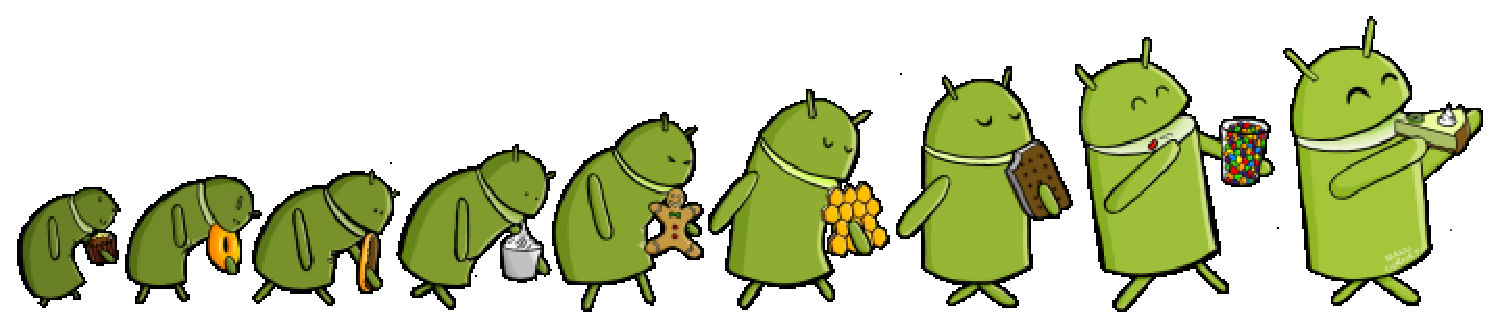
\includegraphics[width=0.9\textwidth]
{imagini/androidVersions.eps}
\end{figure}
\end{center}
Dezvoltarea sistemul de operare Android a început în 2003 de Android Inc. care a fost apoi cumpărat de Google in 2005.[3]
Cea mai recentă actualizare a sistemului Android este versiunea Android 5.0 ,,Lollipop'', care a fost lansată în 3 Noiembrie 2014. Începând cu Aprilie 2009, versiunile Android au fost denumite cu nume de deserturi, fiind lansate în ordine alfabetică, începand cu Android 1.5 ``Cupcake'', versiunile anterioare 1.0 Alpha si 1.1 Beta fiind versiuni pre-comerciale.\cite{9}\newline
\begin{center}
\begin{table}\includegraphics[width=0.9\textwidth, height=0.8\textheight]
\begin{tabular}{|p{5cm}|p{1.5cm}|p{3cm}|p{1.5cm}|}\hiderowcolors
\hline
\cellcolor{LightPink} Data lansării & \cellcolor{LightGreen} Versiune & \cellcolor{LightPink} Nume  & \cellcolor{LightGreen} Nivel API \\
September 2008& 1.0& -- & 1\\
\hline
February 2009& 1.1& -- & 2\\
\hline
April 2009& 1.5& Cupcake& 3\\
\hline
September 2009&1.6& Donut& 4\\
\hline
October 2009& 2.0& Éclair& 5\\
\hline
December 2009& 2.0.1& Éclair& 6\\
\hline
January 2010& 2.1& Éclair& 7\\
\hline
May 2010& 2.2–2.2.3& Froyo& 8\\
\hline
December 2010& 2.3–2.3.2& Gingerbread& 9\\
\hline
February 2011& 2.3.3–2.3.7& Gingerbread& 10\\
\hline
February 2011& 3.0& Honeycomb& 11\\
\hline
May 2011& 3.1& Honeycomb&12\\
\hline
July 2011& 3.2–3.2.6& Honeycomb& 13\\
\hline
October 2011& 4.0–4.0.2& Ice Cream Sandwich& 14\\
\hline
December 2011& 4.0.3–4.0.4& Ice Cream Sandwich& 15\\
\hline
July 2012& 4.1–4.1.2& Jelly Bean& 16\\
\hline
November 2012& 4.2–4.2.2& Jelly Bean& 17\\
\hline
July 2013& 4.3–4.3.1& Jelly Bean& 18\\
\hline
October 2013& 4.4–4.4.4& KitKat& 19\\
\hline
July 2014& 4.4w& KitKat with Wearable Extensions& 20\\
\hline
November 2014& 5.0& Lollipop& 21\\
\hline
\end{tabular}
\caption{Versiuni Android}
\end{table}
\end{center}
În 3 septembrie 2013, Google anuntă că un miliard de dispozitive Android activate sunt folosite în toată lumea. \newline 
În Ianuarie 2015, Android deține 62\% din piața de smartphone-uri și tablete din US, 82.7\% din piața chineză și 73.3\% din piața europeană. \cite{9} \newpage

\section{Android Platform Fragmentation}
La o simplă vedere a datelor de lansare prezentate in tabelul 1-1, este posibil sa credeți că cele mai multe dispozitive Android ruleaza pe minim versiunea Android 4.4, însă acest lucru nu este adevărat. \newline 
Datorită fragmentării mari, datele de lansare nu oferă o imagine clară a ecosistemului Android.\newline 
Tabelul 1 este cel mai recent grafic de distribuție a versiunilor de Android Dashboard2 \cite{2} pe baza datelor colectate în luna decembrie 2014.\cite{1}\newline 


\begin{table}[!hp]
\caption{Distribuția versiunilor Android}
\begin{tabular}{|c|c|c|c|}
\hline
\cellcolor{LightPink}Versiune & \cellcolor{LightGreen} Nume versiune & \cellcolor{LightPink} Nivel API &\cellcolor{LightGreen} Nivel distribuție\\
\hline
2.2–2.2.3& Froyo& 8& 0.5\%\\
\hline
2.3.3–2.3.7& Gingerbread& 9& 9.1\%\\
\hline
4.0.3–4.0.4& Ice Cream Sandwich& 15& 7.8\%\\
\hline
4.1–4.1.2& Jelly Bean& 16& 21.3\%\\
\hline
4.2–4.2.2& Jelly Bean& 17& 20.4\%\\
\hline
4.3–4.3.1& Jelly Bean& 18& 7.0\%\\
\hline
4.4–4.4.4& KitKat& 19& 33.9\%\\
\hline
\end{tabular}
\end{table}


După cum se observă în tabelul 1-2, versiunea de Android 4.4 cuprinde doar sistemele de operare ale 33.9\% de utilizatori din numărul total al acestora. Dezvoltarea unei aplicații Android având ca target doar nivelul API 19 va limita audiența la numai 33.9\% dintre utilizatorii de bază Android.
\newline Cu toate că un nivel API superior furnizeaza funcționalităti suplimentare, este de preferat sa luăm în calcul diagrama de distribuție pentru a determina numărul audienței.\cite{1}

\section{Android Support Library}
Chiar dacă setarea unui target API mai mic mărește numărul de persoane care vor putea utiliza aplicația, de asemenea limitează funcționalitățile de care putem să ne folosim în dezvoltarea unei aplicații Android. Pentru a remedia această problemă, a fost introdus Android Support Library.
Acest pachet pune la dispoziție versiuni anterioare compatibile ale API-urilor recente.\newline 
Acest lucru inseamnă că o aplicație care este dezvoltata pentru nivelul API 19 poate avea ca target nivelele API 4 și nivelurile următoare.\newline 
Includerea bibliotecii Android Support Library într-o aplicație este considerată o tehnică ,,best practice''.\cite{1}
